%%%%%%%%%%%%%%%%%%%%%%%%%%%%%%%%%%%%%%%%%%
\section{Results}
\label{sec:results}

All experiments were executed for 31 independent runs per (configuration, instance) pair. Statistical summaries report mean, median, standard deviation, interquartile range, and coefficient of variation of the final best fitness. Normalized gap was computed as $(\text{fitness}_{\text{best}} - \text{optimum}) / \max(|\text{optimum}|, 1)$, clipped to zero when the optimum was reached. Configuration rankings were compared with a Friedman omnibus test and Nemenyi post-hoc procedure. Run-level RQ4 and rule-pattern comparisons use two-sided independent-sample Mann--Whitney $U$ tests; multiplicity is controlled separately with Bonferroni and Holm correction, respectively. Effect size is summarized with Vargha--Delaney $A_{12}$.

\subsection{Global ranking of fuzzy-control configurations}
\label{subsec:results_global}

Table~\ref{tab:top_configs} ranks the top 10 configurations by mean Friedman rank across all 62 function--dimension instances of F1--F23. The fuzzy configuration \texttt{FCS-3-R1} (three linguistic labels, rule pattern R1) obtained the lowest mean rank (4.77), followed by classical PSO (6.36). Although \texttt{FCS-3-R1} leads the descriptive ranking, the difference between these two configurations is smaller than the Nemenyi critical difference at $\alpha=0.05$. Therefore, the global post-hoc comparison does not establish a statistically significant advantage of \texttt{FCS-3-R1} over classical PSO.


\begin{table}[h]
\centering
\caption{Top 10 of the 33 configurations by mean Friedman rank over 62 benchmark instances (lower is better).}
\label{tab:top_configs}
\begin{tabular}{ll}
\toprule
Configuration & Mean rank \\
\midrule
FCS-3-R1 & 4.774 \\
PSO & 6.363 \\
FCS-5-R1 & 6.968 \\
FCS-7-R1 & 8.202 \\
FCS-9-R1 & 8.427 \\
FCS-9-R5 & 9.016 \\
FCS-3-R5 & 9.250 \\
FCS-7-R5 & 10.129 \\
FCS-3-R6 & 10.694 \\
FCS-5-R5 & 11.565 \\
\bottomrule
\end{tabular}
\end{table}


Table~\ref{tab:hypothesis_summary} summarizes RQ1--RQ5 and their principal evidence, findings, and scope. The Results sections report the global Friedman/Nemenyi comparison, class and subset rank transfer, descriptive dispersion across granularity and rule patterns, independent-sample outcomes against PSO, and subset specialists.

\begin{table}[h]
\centering
\caption{Summary of hypotheses H1--H5 with their governing statistic and verdict.}
\label{tab:hypothesis_summary}
\begin{tabular}{llll}
\toprule
Hypothesis & Statement & Key statistic & Verdict \\
\midrule
H1 & Granularity has diminishing returns & Friedman chi2 p=2.65e-200 & H0 rejected globally; within R1 the effect of n is \textless{} CD (not sig.) \\
H2 & Best R depends on problem class & tau(composed, unimodal)=0.08 & supported \\
H3 & Sensitivity to R decreases with n & n x R SRH p=0.34; peta\textasciicircum{}2(R)=0.063, peta\textasciicircum{}2(n)=0.0007 & rejected \\
H4 & PSO\_FCS beats PSO on \textgreater{}=50\% of instances & best config: 27 wins / 33 ties / 2 losses (of 62) & rejected under strict \textgreater{}=50\% criterion; supported = False \\
H5 & No static (n*, R*) dominates both S1 and S2 & tau(S1, S2)=0.09; argmin(S1)=PSO\_FCS:O1:3:I1:R5, argmin(S2)=PSO\_FCS:O1:5:I1:R6 & supported \\
\bottomrule
\end{tabular}
\end{table}


The Critical Difference diagram in Figure~\ref{fig:fig_cd_diagram_h1} summarizes the Nemenyi post-hoc comparisons. Configurations are ordered by mean rank, and the shaded band identifies those within one critical difference of the leading configuration. Nine configurations fall within this band, including classical PSO. In particular, the mean-rank difference between \texttt{FCS-3-R1} and PSO is 1.59, below the critical difference of 6.59, so their ranking difference is not statistically significant at $\alpha=0.05$. The four R1 variants and four configurations belonging to the R5 and R6 families also fall within the band. In contrast, all configurations based on R2, R3, R4, R7, and R8 lie outside it, with \texttt{FCS-9-R2} ranking last (26.54). These results highlight the relevance of rule-base structure: the four R1 configurations span mean ranks from 4.77 to 8.43, whereas configurations with $n=9$ range from 8.43 to 26.54 depending on the rule pattern. Thus, increasing linguistic resolution does not compensate for differences associated with the consequent mapping in the evaluated controllers.


\begin{figure}[!htbp]
  \begin{adjustwidth}{-\extralength}{0cm}
  \centering
  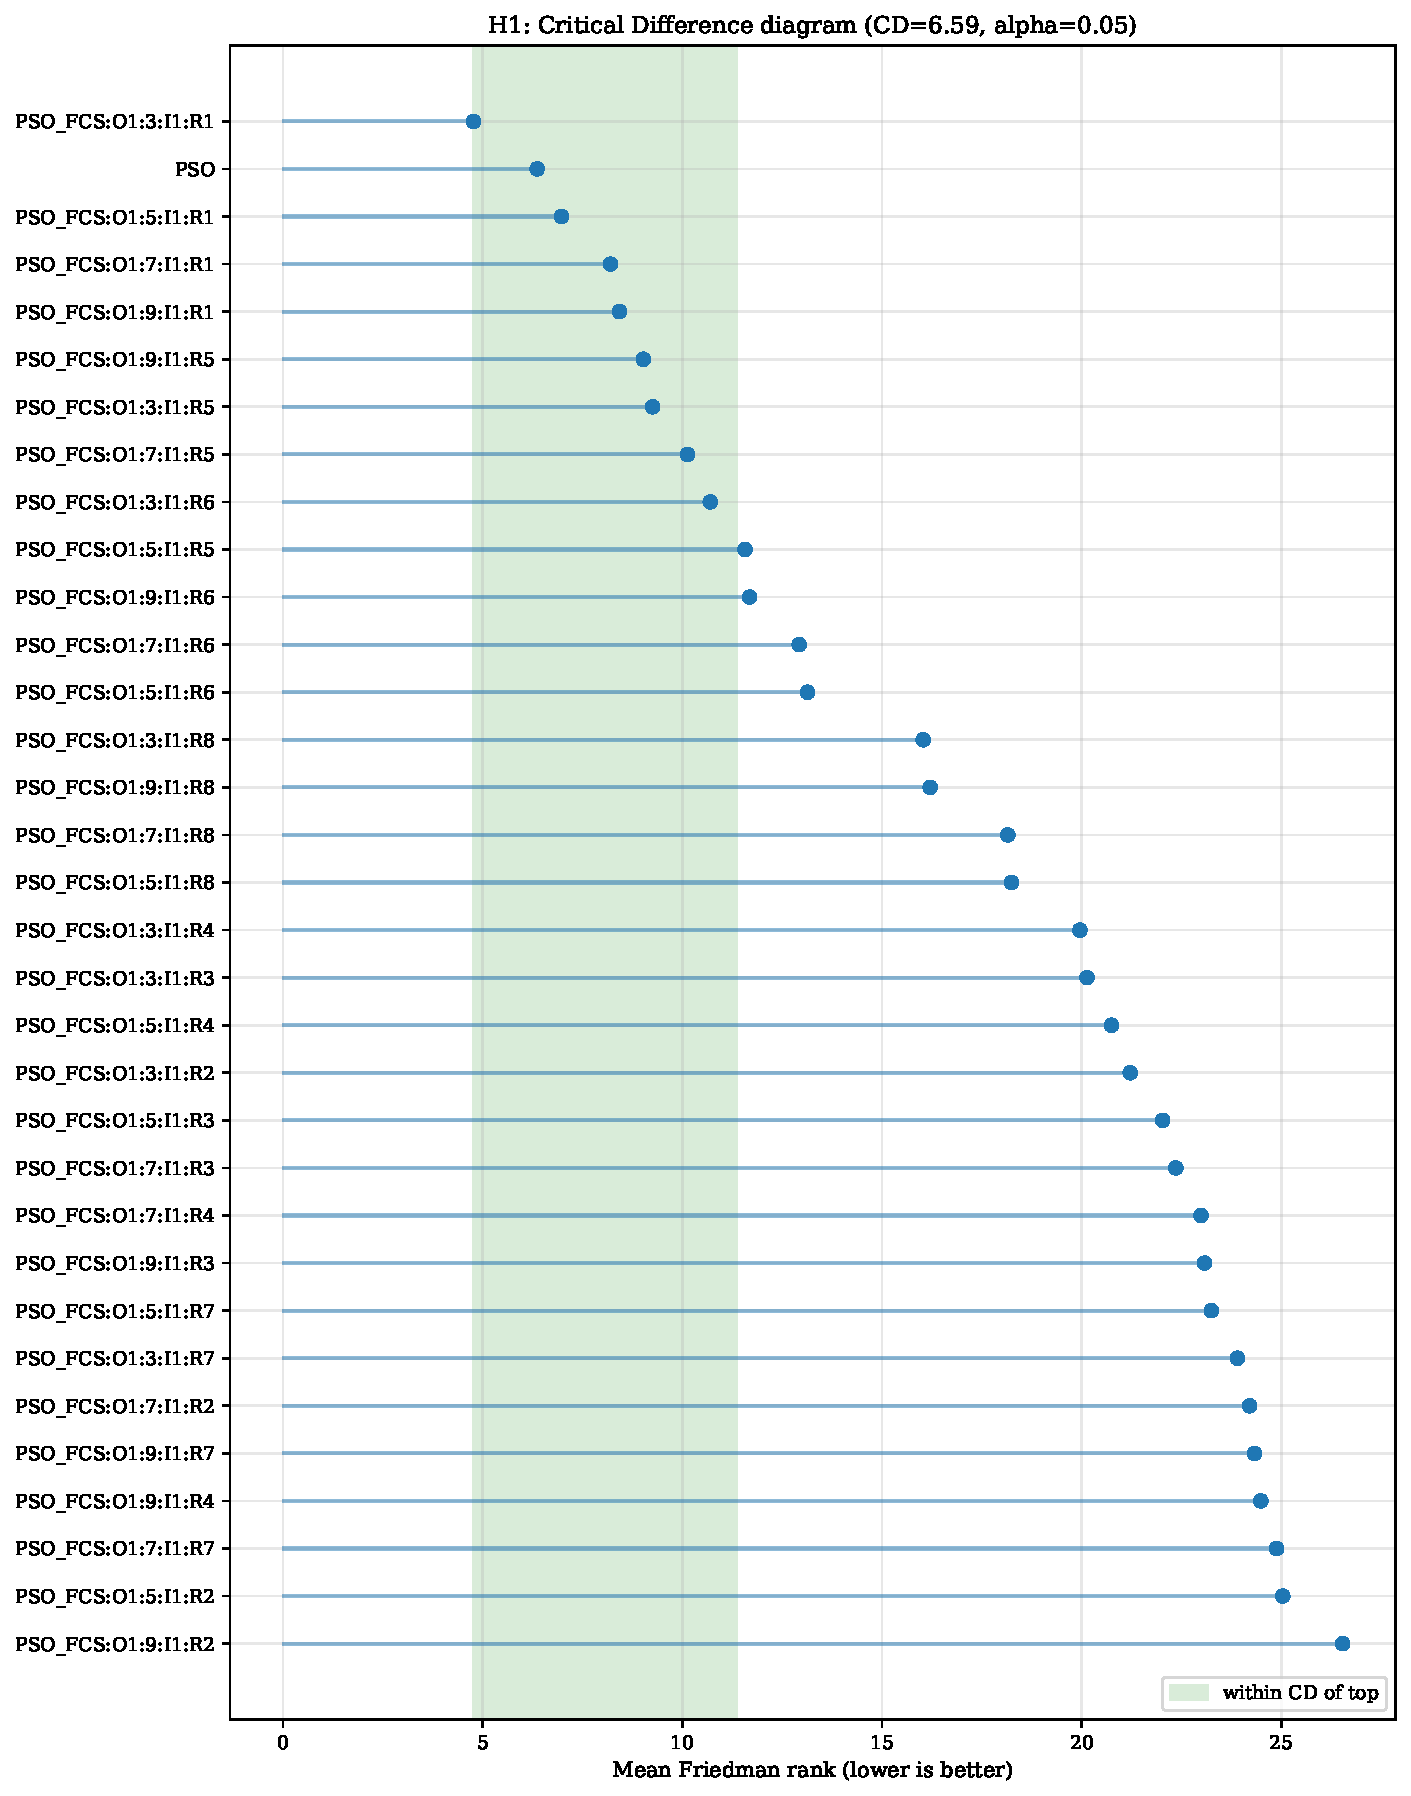
\includegraphics[width=\fulllength,height=0.90\textheight,keepaspectratio]{figures/fig_cd_diagram_h1.pdf}
  \end{adjustwidth}
  \caption{Critical-difference diagram of 33 configurations over 62 instances (Friedman/Nemenyi, $\alpha=0.05$). Lower mean rank is better; shading marks configurations within CD $=6.59$ of the leader. PSO is bold.}
  \label{fig:fig_cd_diagram_h1}
\end{figure}

\subsection{Function-level performance}
\label{subsec:results_function}

The aggregated ranking of Section~\ref{subsec:results_global} hides where each configuration actually wins. Table~\ref{tab:function_level} therefore reports, for every benchmark function, the fuzzy configuration that wins the largest number of its instances, the per-instance rank of that configuration and of the baseline, and the Bonferroni-significant outcomes for the selected configuration. Ranks are computed within each instance over the 33 algorithmic configurations using the median normalized gap, so rank~1 denotes the best configuration on that instance. Configurations are named \texttt{FCS-$n$-R$k$}, where $n$ is the number of linguistic labels and $k$ the rule-base pattern; the input and output partition families are I1 and O1 for every configuration and are therefore omitted from the label.

\afterpage{\startlandscape
\begin{table}[H]
\centering
\small
\caption{Function-level summary of the FCS configuration with the most per-instance rank wins, its ranks, Bonferroni-significant outcomes, effect size, and unpaired runtime overhead.}
\label{tab:function_level}
\setlength{\tabcolsep}{3pt}
\begin{tabular*}{\textwidth}{@{\extracolsep{\fill}}l p{2.8cm} p{1.9cm} p{2.1cm} c c c c c c}
\toprule
\textbf{Function} & \textbf{Landscape} & \textbf{Dimensions} & \textbf{Best FCS} & \textbf{PSO rank} & \textbf{FCS rank} & \textbf{Rank wins} & \textbf{Bonferroni wins} & \boldmath$A_{12}$ & \textbf{Overhead (\%)} \\
\midrule
F1 & Unimodal & 10, 30, 50, 100 & \texttt{FCS-3-R1} & 3.0 & 1.0 & 4/4 & 3/4 & 0.96 & 31.8 \\
F2 & Unimodal & 10, 30, 50, 100 & \texttt{FCS-3-R1} & 2.0 & 1.0 & 4/4 & 4/4 & 0.98 & 34.1 \\
F3 & Unimodal & 10, 30, 50, 100 & \texttt{FCS-5-R5} & 11.0 & 1.0 & 4/4 & 1/4 & 0.74 & 14.6 \\
F4 & Unimodal & 10, 30, 50, 100 & \texttt{FCS-9-R5} & 4.0 & 1.0 & 3/4 & 1/4 & 0.56 & 26.2 \\
F5 & Unimodal & 10, 30, 50, 100 & \texttt{FCS-3-R1} & 3.0 & 1.0 & 4/4 & 0/4 & 0.64 & 29.6 \\
F6 & Unimodal & 10, 30, 50, 100 & \texttt{FCS-3-R1} & 2.0 & 1.0 & 4/4 & 4/4 & 0.95 & 33.9 \\
F7 & Unimodal & 10, 30, 50, 100 & \texttt{FCS-5-R1} & 3.0 & 1.0 & 3/4 & 0/4 & 0.54 & 28.7 \\
\midrule
F8 & Scalable multimodal & 10, 30, 50, 100 & \texttt{FCS-9-R8} & 3.5 & 1.5 & 2/4 & 0/4 & 0.54 & 27.1 \\
F9 & Scalable multimodal & 10, 30, 50, 100 & \texttt{FCS-5-R2} & 9.0 & 1.0 & 4/4 & 0/4 & 0.60 & 25.4 \\
F10 & Scalable multimodal & 10, 30, 50, 100 & \texttt{FCS-3-R1} & 3.5 & 1.0 & 3/4 & 1/4 & 0.77 & 26.9 \\
F11 & Scalable multimodal & 10, 30, 50, 100 & \texttt{FCS-3-R1} & 4.0 & 1.0 & 4/4 & 2/4 & 0.75 & 30.7 \\
F12 & Scalable multimodal & 10, 30, 50, 100 & \texttt{FCS-3-R1} & 2.0 & 1.0 & 3/4 & 0/4 & 0.72 & 25.4 \\
F13 & Scalable multimodal & 10, 30, 50, 100 & \texttt{FCS-3-R1} & 3.0 & 1.0 & 4/4 & 0/4 & 0.74 & 28.7 \\
\midrule
F14 & Fixed-dimensional & 2 & \texttt{FCS-3-R1} & 27.0 & 3.0 & 1/1 & 0/1 & 0.58 & -5.0 \\
F15 & Fixed-dimensional & 4 & \texttt{FCS-3-R1} & 11.0 & 1.0 & 1/1 & 0/1 & 0.75 & 86.9 \\
F16 & Fixed-dimensional & 2 & -- & 17.0 & 17.0 & 0/1 & 0/1 & 0.56 & -- \\
F17 & Fixed-dimensional & 2 & -- & 17.0 & 17.0 & 0/1 & 0/1 & 0.50 & -- \\
F18 & Fixed-dimensional & 2 & \texttt{FCS-3-R1} & 15.0 & 15.0 & 0/1 & 0/1 & 0.45 & 161.5 \\
F19 & Fixed-dimensional & 3 & -- & 17.0 & 17.0 & 0/1 & 0/1 & 0.56 & -- \\
F20 & Fixed-dimensional & 6 & \texttt{FCS-3-R1} & 14.0 & 14.0 & 0/1 & 0/1 & 0.55 & 53.2 \\
F21 & Fixed-dimensional & 4 & \texttt{FCS-7-R1} & 24.0 & 1.0 & 1/1 & 0/1 & 0.61 & 17.8 \\
F22 & Fixed-dimensional & 4 & \texttt{FCS-3-R6} & 20.0 & 1.0 & 1/1 & 0/1 & 0.57 & 14.6 \\
F23 & Fixed-dimensional & 4 & \texttt{FCS-5-R6} & 1.0 & 2.0 & 0/1 & 0/1 & 0.34 & 8.2 \\
\bottomrule
\end{tabular*}
\noindent\footnotesize
Ranks are medians of per-instance ranks on median normalized gap (lower is better). Rank wins count instances where the selected FCS has a lower rank than PSO. Bonferroni wins use independent-sample Mann--Whitney tests adjusted over all 1,984 RQ4 comparisons. $A_{12}$ is the median effect size; $A_{12}>0.5$ favours FCS. Overhead is $100(\mathrm{median}(t_{\mathrm{FCS}})/\mathrm{median}(t_{\mathrm{PSO}})-1)$ using independent run samples. A dash marks functions where all FCS configurations share the best median-gap rank.
\end{table}
\finishlandscape
\restoreportraitheight}

Three observations follow from the disaggregated view. First, the best fuzzy configuration outranks the baseline on 50 of the 62 instances. Of these rank wins, 32 have nominal independent-sample $p<0.05$ and 17 remain significant after Bonferroni correction across the RQ4 family. The baseline ranks ahead on 6 instances, and the best FCS and PSO share the minimum rank on the remaining 6. Second, the winning configuration is not unique: 15 distinct FCS configurations record at least one rank-based win over PSO. \texttt{FCS-3-R1} accounts for 30 of the 50 wins, including 28 of the 46 wins in the scalable subset $S_1$; the other wins span all four granularities and six additional rule patterns. The function-level table identifies the best fuzzy candidate even when it does not outrank PSO. Third, the effect size is heterogeneous: the median $A_{12}$ reaches 0.95--0.98 on F1, F2, and F6, but remains near 0.54 on F7 and F8 and on most fixed-dimensional functions.

The fixed-dimensional subset behaves differently from the scalable one. On F16 and F17, normalized gap is zero in all 31 runs for all 33 configurations. On F19, 990 of 1023 run-level gaps are zero; although 33 runs have a nonzero gap, every configuration has a zero median gap. The 33 configurations therefore share mean rank 17 on these functions, and no unique median-gap winner is identified. For F16, the independent-sample test on raw final fitness is nominally significant ($p=0.0419$), but its Bonferroni-adjusted $p$ is 1.000; $A_{12}=0.56$ and all normalized gaps are zero, so the test does not establish a normalized-gap advantage. On F14, F15, F21, and F22 the baseline falls to ranks 11--27 while a fuzzy configuration takes the first position. On F23, the ordering reverses: PSO takes the first position and the best fuzzy configuration, \texttt{FCS-5-R6}, ranks second with $A_{12}=0.34$, favouring PSO. The independent-sample $p=0.0234$ is nominally significant but does not survive Bonferroni correction. This subset therefore includes both large rank differences favouring fuzzy control and a function on which PSO ranks first; it does not support a universally dominant configuration.

Figure~\ref{fig:fig_function_heatmap} in Appendix~\ref{app:instance_results} shows the complete rank matrix: columns are ordered by mean rank, PSO is bracketed, and the S1/S2 boundary is marked. It shows predominantly better FCS ranks across the scalable subset and more varied outcomes across fixed-dimensional instances, complementing Table~\ref{tab:function_level}.

\subsection{Problem-class dependence}
\label{subsec:results_class}

Across the evaluated configurations, performance rankings show greater variation among rule-base patterns (R1--R8) than among linguistic granularities ($n \in \{3,5,7,9\}$). Figure~\ref{fig:fig_rule_class_heatmap} presents, for each configuration and landscape class, the mean across instances of the instance-level median normalized gap (smaller is better). The classes are unimodal functions (F1--F7), scalable multimodal functions (F8--F13), and fixed-dimensional multimodal functions (F14--F23); each configuration appears once as a row.

\begin{figure}[!htbp]
  \centering
  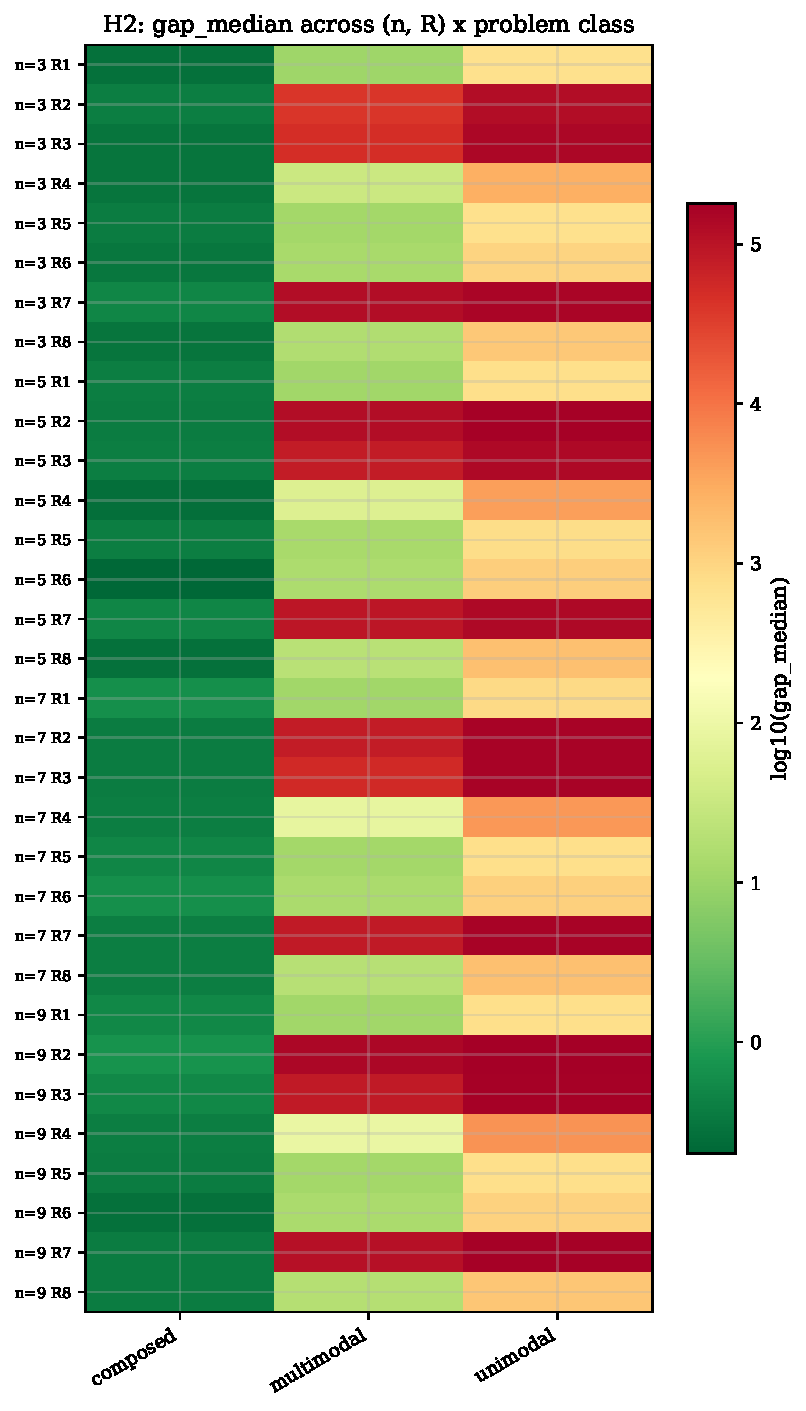
\includegraphics[width=0.65\linewidth]{figures/fig_rule_class_heatmap.pdf}
  \caption{Mean instance-level median normalized gap for the 32 FCS configurations by landscape class. Colour shows $\log_{10}$ mean gap with a $10^{-12}$ display floor; lower values indicate better performance.}
  \label{fig:fig_rule_class_heatmap}
\end{figure}

Two complementary partitions of the benchmark are used. For landscape effects, functions are grouped as unimodal (F1--F7), scalable multimodal (F8--F13), and fixed-dimensional multimodal (F14--F23). For the transferability analysis, the benchmark is split into the scalable subset $S_1$ (F1--F13, evaluated at four dimensions each) and the fixed-dimensional subset $S_2$ (F14--F23); this split is by dimensional regime, not by modality.

Table~\ref{tab:class_summary} summarizes the class-level rankings. The leading configuration differs across the evaluated groups: \texttt{FCS-3-R5} leads on unimodal functions, \texttt{FCS-3-R1} on scalable multimodal functions, and \texttt{FCS-5-R6} on fixed-dimensional functions. \texttt{FCS-3-R1} remains relatively competitive, ranking 2nd, 1st, and 3rd, respectively. These descriptive results do not isolate causal effects of modality or dimensionality, nor establish a universally optimal configuration for any group.

\begin{table}[!htbp]
\centering
\small
\caption{Positions of the 33 configurations by mean instance-level median normalized gap within each benchmark group (lower is better). For each configuration--instance pair, the median normalized gap over 31 runs was first computed; these medians were then averaged within the group. Positions use minimum ranks for ties and are not Friedman mean ranks.}
\label{tab:class_summary}
\setlength{\tabcolsep}{3pt}
\begin{tabularx}{\textwidth}{@{}>{\raggedright\arraybackslash}Xcc>{\raggedright\arraybackslash}p{2.7cm}cc@{}}
\toprule
\textbf{Benchmark group} & \textbf{Functions} & \textbf{Instances} & 
\textbf{Leading configuration} & \textbf{PSO position} & \textbf{FCS-3-R1 position} \\
\midrule
Unimodal (F1--F7) & 7 & 28 & FCS-3-R5 & 8/33 & 2/33 \\
Scalable multimodal (F8--F13) & 6 & 24 & FCS-3-R1 & 2/33 & 1/33 \\
Fixed-dimensional (F14--F23) & 10 & 10 & FCS-5-R6 & 25/33 & 3/33 \\
\bottomrule
\end{tabularx}
\end{table}


As a descriptive sensitivity check, configurations were also ranked by median normalized gap within each instance and these ranks were averaged by benchmark group. Under mean within-instance ranks, FCS-3-R1 leads the unimodal group (with PSO 2nd and FCS-3-R1 1st), remains the scalable multimodal leader (PSO 2nd and FCS-3-R1 1st), and FCS-5-R6 remains the fixed-dimensional leader (PSO 17th and FCS-3-R1 2nd). The unimodal leader therefore changes from FCS-3-R5 under mean instance-level median gap to FCS-3-R1 under mean within-instance rank. The gap mean preserves magnitude differences among instances, whereas the rank mean summarizes relative ordering with equal instance weight; neither aggregation is universally superior.

Table~\ref{tab:kendall_class} reports Kendall $\tau$ between the configuration rankings induced by each pair of landscape classes. The two scalable classes show strong observed rank concordance ($\tau=0.867$ between unimodal and scalable multimodal); the fixed-dimensional class shows weak observed concordance with them ($\tau=0.080$ and $\tau=0.083$). These coefficients describe the evaluated classes and do not establish independence or a general transferability result.

\begin{table}[h]
\centering
\caption{Kendall's tau between rankings induced by the three problem classes (higher = more agreement).}
\label{tab:kendall_class}
\begin{tabular}{llll}
\toprule
class & composed & multimodal & unimodal \\
\midrule
composed & 1.000 & 0.080 & 0.083 \\
multimodal & 0.080 & 1.000 & 0.867 \\
unimodal & 0.083 & 0.867 & 1.000 \\
\bottomrule
\end{tabular}
\end{table}


Rank concordance between $S_1$ and $S_2$ is weak ($\tau=0.095$, $p=0.451$); this non-significant result does not establish independence. \texttt{FCS-3-R5} has the lowest mean normalized gap on $S_1$ and ranks 11th on $S_2$, whereas \texttt{FCS-5-R6} leads on $S_2$ and ranks 13th on $S_1$. These rankings describe only the evaluated subsets.

Figure~\ref{fig:fig_pareto_s1_s2} plots the configuration ranks in the $(S_1,S_2)$ space and highlights the non-dominated frontier. No configuration achieves the best rank on both subsets: the frontier includes the two subset specialists and \texttt{FCS-3-R1}, which ranks second on S1 and third on S2 and offers the closest observed compromise. This dispersion is the aggregated counterpart of the per-instance heterogeneity reported in Section~\ref{subsec:results_function}.


\begin{figure}[!h]
  \centering
  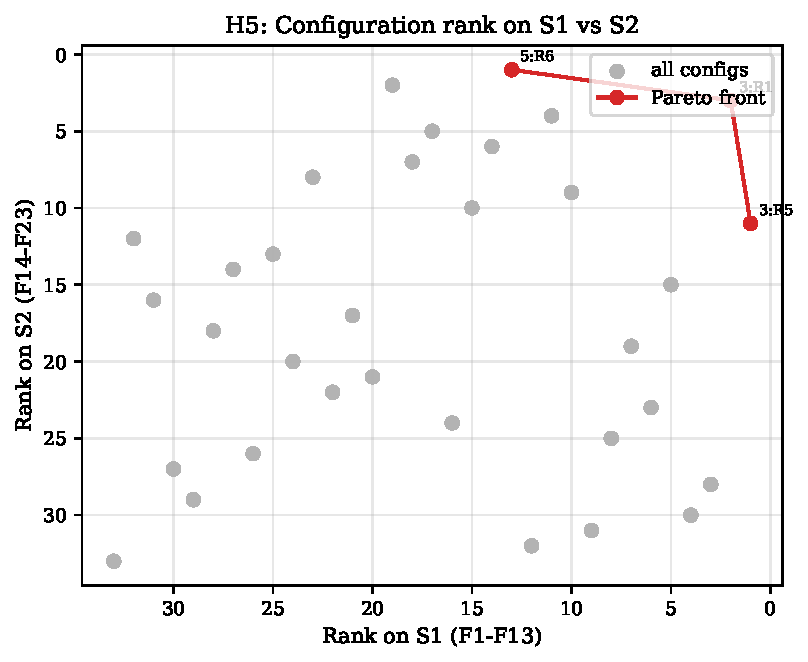
\includegraphics[width=0.85\linewidth]{figures/fig_pareto_s1_s2.pdf}
  \caption{Configuration ranks on S1 versus S2, computed from per-instance median normalized gap; better ranks lie toward the upper right. The red line marks the non-dominated frontier and the star denotes PSO.}
  \label{fig:fig_pareto_s1_s2}
\end{figure}

\subsection{Effect of rule-base structure}
\label{subsec:results_rules}

Sections~\ref{subsec:results_global}--\ref{subsec:results_class} establish that rule-table patterns separate the configurations more sharply than the number of labels, but do not by themselves attribute this ranking to independent input effects. As defined in Section~\ref{subsec:formal_rules}, R1--R8 combine two nominal consequent axes: progress direction (decreasing, neutral, or increasing) and diversity reaction (following, neutral, or compensating). Table~\ref{tab:rule_semantic_grid} places the patterns on those axes with their mean Friedman rank across the four granularities. A neutral consequent axis does not guarantee that the corresponding input is absent from the effective Mamdani surface.

\begin{table}[H]
\centering
\small
\caption{Mean Friedman ranks by nominal progress direction and diversity consequent, averaged over four granularities. A neutral consequent does not remove an antecedent from Mamdani inference.}
\label{tab:rule_semantic_grid}
\begin{tabular}{lccc}
\toprule
 & \textbf{Diversity-following} & \textbf{Diversity-neutral} & \textbf{Diversity-compensating} \\
\midrule
\textbf{Progress decreasing} & R5 (10.0) & R1 (7.1) & R6 (12.1) \\
\textbf{Progress neutral} & R3 (21.9) & -- & R4 (22.0) \\
\textbf{Progress increasing} & R7 (24.1) & R2 (24.3) & R8 (17.2) \\
\bottomrule
\end{tabular}
\end{table}


The grid is ordered almost entirely by rows. The three patterns with a decreasing progress effect occupy the best mean ranks (R1 = 7.1, R5 = 10.0, R6 = 12.1), the two progress-neutral patterns sit in the lower half (R3 = 21.9, R4 = 22.0), and two of the three patterns with an increasing progress effect close the ranking (R7 = 24.1, R2 = 24.3). Column position accounts for a much smaller spread: within the decreasing row the three patterns differ by 5.0 ranks, whereas the difference between the best and the worst row exceeds 17 ranks.

To compare rule-pattern contrasts, the 31 run-level outcomes for each pattern are treated as independent samples at equal granularity and on the same instance. The two-sided Mann--Whitney tests are adjusted with Holm's procedure across all 1,984 contrasts. Mirror pairs invert every non-neutral consequent axis and, by Proposition~\ref{prop:mirror}, reflect the control surface about the midpoint of $[w_{\min},w_{\max}]$. Single-axis pairs change one nominal consequent axis while holding the other fixed. These are descriptive comparisons of rule tables; they do not imply orthogonal effective-input effects under min--max inference. Table~\ref{tab:rule_pairs} reports both pair families.

\begin{table}[!htbp]
\centering
\small
\caption{Independent-sample comparisons of rule-pattern pairs at equal granularity and instance (248 tests per pair). Holm adjustment is applied once across the complete family of 1,984 comparisons.}
\label{tab:rule_pairs}
\begin{adjustwidth}{-\extralength}{0cm}
\setlength{\tabcolsep}{4pt}
\renewcommand{\arraystretch}{1.15}
\renewcommand{\tabularxcolumn}[1]{m{#1}}
\begin{tabularx}{\fulllength}{@{}l>{\raggedright\arraybackslash}X c c c c l@{}}
\toprule
\textbf{Pair} & \textbf{Axis changed} & \textbf{Nominal W/NS/L} & \textbf{Holm W/NS/L} & \textbf{Dominant} & \boldmath$A_{12}$ & \textbf{Strongest in} \\
\midrule
\multicolumn{7}{l}{\emph{Mirror pairs}} \\
R1 vs R2 & progress direction & 192/56/0 & 175/73/0 & \textbf{R1} & 0.99 & Unimodal \\
R3 vs R4 & diversity reaction & 118/59/71 & 104/98/46 & \textbf{R4} & 0.41 & Scalable multimodal \\
R5 vs R8 & progress direction + diversity reaction & 173/73/2 & 142/106/0 & \textbf{R5} & 0.91 & Unimodal \\
R6 vs R7 & progress direction + diversity reaction & 173/57/18 & 152/91/5 & \textbf{R6} & 0.95 & Scalable multimodal \\
\midrule
\multicolumn{7}{l}{\emph{Single-axis pairs}} \\
R5 vs R7 & progress direction & 172/75/1 & 152/96/0 & \textbf{R5} & 0.96 & Scalable multimodal \\
R6 vs R8 & progress direction & 176/65/7 & 156/92/0 & \textbf{R6} & 0.92 & Unimodal \\
R5 vs R6 & diversity reaction & 132/81/35 & 99/130/19 & \textbf{R5} & 0.66 & Unimodal \\
R7 vs R8 & diversity reaction & 154/68/26 & 137/98/13 & \textbf{R8} & 0.09 & Scalable multimodal \\
\bottomrule
\end{tabularx}
\noindent\footnotesize
W/NS/L denotes significant wins for the dominant pattern, non-significant comparisons, and significant losses. Nominal counts use $p<0.05$; Holm counts use adjusted $p<0.05$ across all 1,984 tests. $A_{12}$ is the median effect for the first pattern; values above 0.5 favour it. These contrasts compare implemented rule tables and do not isolate causal input effects.
\end{adjustwidth}
\end{table}


After Holm correction across the full Table 11 family, the decreasing-progress pattern has more significant wins than losses in each matched contrast with its increasing-progress counterpart: R1 over R2, 175/73/0 (wins/non-significant/losses); R5 over R7, 152/96/0; and R6 over R8, 156/92/0. Their median $A_{12}$ values are 0.99, 0.96, and 0.92, respectively. These are empirical differences among the tested rule tables, not evidence that the effective controller responds only to progress.

Among patterns with different diversity consequents, the Holm-adjusted independent-sample comparisons also vary with the nominal progress direction. For decreasing progress, R5 has 99 significant wins and 19 losses against R6, with 130 non-significant comparisons ($A_{12}=0.66$). For increasing progress, R8 has 137 wins and 13 losses against R7, with 98 non-significant comparisons ($A_{12}=0.09$ in favour of R8). For the nominally progress-neutral pattern, R4 has 104 wins and 46 losses against R3, with 98 non-significant comparisons; their aggregate mean ranks remain close (22.0 and 21.9). These comparisons describe the tested rule tables and do not establish a general benefit of diversity feedback.

Both effects are also visible in the mirror pairs, which reverse the pattern as a whole. R1 dominates R2 and R5 dominates R8 most clearly on the unimodal class, whereas R6 dominates R7 most clearly on the scalable multimodal class, which is consistent with the landscape dependence reported in Section~\ref{subsec:results_class}.

These results explain the composition of the leading group of Section~\ref{subsec:results_global}. Every configuration inside the critical-difference band uses a decreasing-progress consequent pattern: the four R1 variants, three R5 variants, and one R6 variant. No pattern with a nominally neutral or increasing progress consequent enters the band, and R2, R3, R4, R7, and R8 remain outside it at every granularity. The single exception to the row ordering, R8 at rank 17.2 ahead of the nominally progress-neutral R3 and R4, combines an increasing-progress consequent with the compensating diversity consequent favoured by the Holm-adjusted R7--R8 contrast. Overall, rankings align most strongly with nominal progress-consequent direction, while independent-sample differences across diversity-consequent patterns depend on that direction. Since a neutral consequent axis does not remove the input from min--max firing, these comparisons are not independent causal effects of the two inputs.

\subsection{Effect of linguistic granularity}
\label{subsec:results_granularity}

Granularity cannot be read in isolation from the rule-base pattern, because $n$ fixes the resolution at which a pattern is expressed and simultaneously raises the number of consequents from $n^2 = 9$ at $n=3$ to $n^2 = 81$ at $n=9$. Table~\ref{tab:granularity_by_rule} therefore reports the mean Friedman rank of every pattern at each granularity, together with the granularity that minimizes it and the spread between its best and worst rank.

\begin{table}[H]
\centering
\small
\caption{Mean Friedman rank of each rule-base pattern at each granularity (lower is better). Spread is the maximum minus minimum across $n$; the 2.5-rank stability threshold is descriptive, not an equivalence test.}
\label{tab:granularity_by_rule}
\setlength{\tabcolsep}{3.5pt}
\begin{tabular}{lcccccccl}
\toprule
\textbf{Pattern} & \textbf{Progress} & \boldmath$n=3$ & \boldmath$n=5$ & \boldmath$n=7$ & \boldmath$n=9$ & \textbf{Best} \boldmath$n$ & \textbf{Spread} & \textbf{Trend} \\
\midrule
R1 & dec. & 4.8 & 7.0 & 8.2 & 8.4 & 3 & 3.7 & degradation \\
R2 & incr. & 21.2 & 25.0 & 24.3 & 26.5 & 3 & 5.3 & degrad. (non-monot.) \\
R3 & neutral & 20.1 & 22.0 & 22.4 & 23.1 & 3 & 2.9 & degradation \\
R4 & neutral & 20.0 & 20.8 & 23.0 & 24.5 & 3 & 4.5 & degradation \\
R5 & dec. & 9.2 & 11.6 & 10.1 & 9.0 & 9 & 2.5 & non-monotonic \\
R6 & dec. & 10.7 & 13.1 & 12.9 & 11.7 & 3 & 2.4 & stable \\
R7 & incr. & 23.9 & 23.2 & 24.9 & 24.3 & 5 & 1.6 & stable \\
R8 & incr. & 16.0 & 18.2 & 18.1 & 16.2 & 3 & 2.2 & stable \\
\bottomrule
\end{tabular}
\end{table}


Six of the eight patterns attain their best rank at $n=3$; the exceptions are R5, which is marginally better at $n=9$ (9.02 against 9.25), and R7, which is marginally better at $n=5$ within a spread of 1.6 ranks. The response to $n$ is pattern-dependent. R1's mean rank worsens monotonically from 4.77 at $n=3$ to 8.43 at $n=9$, an increase of 3.65 positions, but this is not the largest change across patterns: R2 increases by 5.33 positions (spread 5.3) and R4 by 4.53 (spread 4.5). Here, spread is the maximum minus minimum mean rank over the four granularities. R6, R7, and R8 show comparatively small observed spreads of 2.4, 1.6, and 2.2 positions, respectively. The table's 2.5-rank stability threshold is descriptive; it does not establish equivalence or absence of a granularity effect.

The aggregate view agrees. Averaged over the eight patterns, the mean rank worsens from 15.74 at $n=3$ to 17.62 at $n=5$ and then remains near 17.99 and 17.97 for $n=7$ and $n=9$; the best rank achievable at each granularity degrades monotonically from 4.77 to 6.97, 8.20, and 8.43. The distribution of the normalized gap, shown in Figure~\ref{fig:fig_boxplot_gap_by_n}, follows the same shape: the median of $\log_{10}$ gap rises from 0.02 at $n=3$ to 0.22 at $n=5$ and then settles at 0.21 and 0.19, while the interquartile range contracts from 3.50 to 3.19 and remains at 3.24 and 3.27. The observed gap worsens from three to five labels and then changes little through $n=9$.

\begin{figure}[!h]
  \centering
  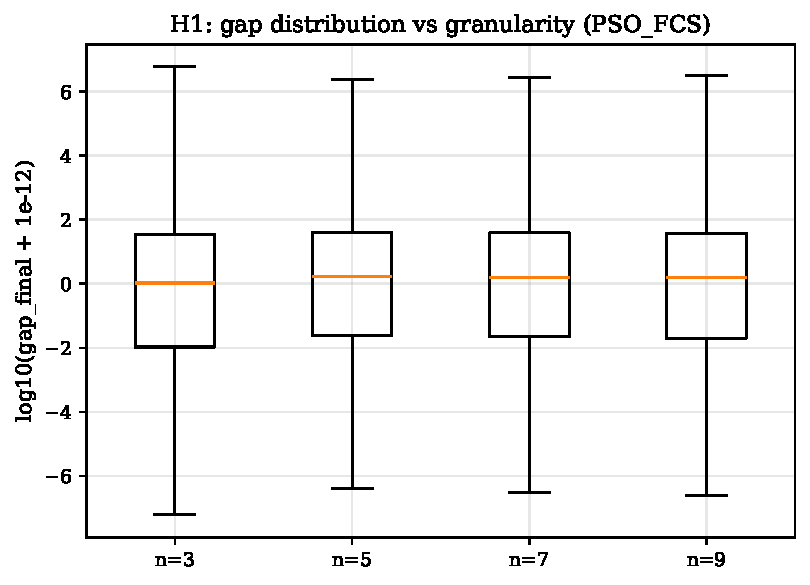
\includegraphics[width=0.85\linewidth]{figures/fig_boxplot_gap_by_n.pdf}
  \caption{Boxplots of run-level final normalized gap, transformed as $\log_{10}(\max(\mathrm{gap},10^{-12})+10^{-12})$ and pooled over 62 instances and eight FCS patterns at each granularity. Outliers are omitted.}
  \label{fig:fig_boxplot_gap_by_n}
\end{figure}

Figure~\ref{fig:fig_granularity_effect} descriptively traces each rule-base pattern across linguistic granularities. Across $n=3$, $5$, $7$, and $9$, the progress-decreasing family remains ahead of the other two nominal consequent-direction families, with R1, R5, and R6 occupying the first three positions at every evaluated granularity. Kendall's $\tau$ between the orderings of the eight patterns at different granularities ranges from 0.79 to 0.93, with the minimum observed between the most distant pair, $n=3$ and $n=9$. Changes in granularity mainly shift the patterns vertically without altering the identity of the leading family; the observed exchanges of position occur within the lower-ranked group outside the critical-difference band, where R2, R3, R4, and R7 interchange positions. These benchmark-wide profiles describe relative ranks and should be distinguished from performance-gap dispersion or a formal interaction effect.

\begin{figure}[!h]
  \centering
  \includegraphics[width=\textwidth]{figures/fig_granularity_effect.pdf}
  \caption{Benchmark-wide summaries over the 62 function--dimension instances. Left: mean Friedman rank by rule-base pattern and linguistic granularity, where better (lower) ranks appear toward the top; colour and line style indicate the nominal direction of the progress consequents. Right: standard deviation across the eight pattern-specific mean ranks for each granularity.}
  \label{fig:fig_granularity_effect}
\end{figure}

In the benchmark-wide summary, the standard deviation across the eight mean Friedman ranks is 6.778, 6.397, 6.707, and 7.524 for $n=3,5,7,9$. The standard deviation across the eight pooled median normalized gaps is 3.994, 4.460, 4.470, and 4.635; these gap medians pool 1,922 run-level observations per pattern and granularity. The median of the function-level rank spreads across the 23 functions is 8.884, 8.366, 8.715, and 9.374; the corresponding log-gap spreads are 0.912, 1.170, 1.173, and 0.901. For ranks, the $S_1$ medians are 8.884, 8.789, 9.128, and 10.194, while the $S_2$ medians are 7.255, 6.556, 6.834, and 5.456. For log-gaps, the $S_1$ medians are 1.359, 1.468, 1.374, and 1.396, and the $S_2$ medians are 0.075, 0.308, 0.263, and 0.070. From $n=3$ to $n=9$, rank spread is lower in 6/23 functions and log-gap spread in 11/23; each measure is non-increasing across all four granularities in 3/23 functions. The observed dispersion therefore does not decrease consistently as linguistic granularity increases. Together with the configuration rankings and pattern-dependent responses reported above, this finding indicates that finer linguistic partitions do not guarantee better optimization performance or more consistent behavior across rule-base patterns. Within the evaluated Mamdani controllers, the organization of the consequent rules remains an important design consideration, rather than linguistic resolution alone. These observations are descriptive and do not establish independent causal effects, statistical equivalence, or a formal granularity-by-rule interaction.


\subsection{Robustness, dimensional scaling, and computational overhead}
\label{subsec:results_robustness}

Section~\ref{subsec:results_function} measured the best fuzzy configuration available on each instance, which is an oracle selection: the winner is allowed to change from one instance to the next. The complementary and stricter question is whether a \emph{single fixed} configuration, chosen once and applied everywhere, beats the baseline across the benchmark. Table~\ref{tab:h4_wilcoxon} reports the ten configurations with the largest number of Bonferroni-significant wins, ordered by corrected wins, nominal wins, and then mean $A_{12}$. Each configuration is compared with PSO on all 62 instances using independent samples and a two-sided Mann--Whitney $U$ test. Because the objective is minimized, the Vargha--Delaney effect size is defined so that $A_{12} > 0.5$ favours the fuzzy configuration and $A_{12} < 0.5$ favours the baseline.

\begin{table}[h]
\centering
\caption{Wilcoxon signed-rank comparison of top-10 PSO\_FCS configurations against classical PSO (paired by run). Columns marked * apply Bonferroni correction over the full 32x62 grid.}
\label{tab:h4_wilcoxon}
\begin{tabular}{llllllllll}
\toprule
Config. & n & R & Wins & Ties & Losses & Wins* & Ties* & Losses* & A12 mean \\
\midrule
PSO\_FCS:O1:3:I1:R1 & 3.000 & R1 & 27 & 33 & 2 & 13 & 49 & 0 & 0.669 \\
PSO\_FCS:O1:7:I1:R5 & 7.000 & R5 & 6 & 28 & 28 & 1 & 43 & 18 & 0.363 \\
PSO\_FCS:O1:9:I1:R5 & 9.000 & R5 & 5 & 31 & 26 & 0 & 47 & 15 & 0.383 \\
PSO\_FCS:O1:5:I1:R5 & 5.000 & R5 & 5 & 24 & 33 & 0 & 38 & 24 & 0.304 \\
PSO\_FCS:O1:5:I1:R1 & 5.000 & R1 & 4 & 51 & 7 & 0 & 62 & 0 & 0.463 \\
PSO\_FCS:O1:3:I1:R5 & 3.000 & R5 & 4 & 27 & 31 & 0 & 48 & 14 & 0.358 \\
PSO\_FCS:O1:9:I1:R1 & 9.000 & R1 & 2 & 53 & 7 & 0 & 62 & 0 & 0.444 \\
PSO\_FCS:O1:7:I1:R7 & 7.000 & R7 & 2 & 14 & 46 & 0 & 23 & 39 & 0.173 \\
PSO\_FCS:O1:7:I1:R1 & 7.000 & R1 & 1 & 55 & 6 & 0 & 62 & 0 & 0.447 \\
PSO\_FCS:O1:3:I1:R6 & 3.000 & R6 & 1 & 23 & 38 & 0 & 35 & 27 & 0.225 \\
\bottomrule
\end{tabular}
\end{table}


The leading fixed configuration, \texttt{FCS-3-R1}, records nominal W/NS/L = 30/30/2 and mean $A_{12}=0.67$; Bonferroni adjustment leaves 16/46/0. The other R1 granularities have 62 non-significant results each after correction, despite nominal non-significant counts of 54, 56, and 53. This is not an equivalence result. Several R5 and R7 variants have more adjusted losses than wins, with mean $A_{12}$ favouring PSO. The 50/62 instance-specific rank wins remain an oracle summary, not a deployable policy.

Figure~\ref{fig:fig_h4_independent_outcomes} presents the nominal comparison outcomes, while Table~\ref{tab:h4_wilcoxon} reports Bonferroni-adjusted results and effect sizes. The supplementary mean--dispersion plots illustrate performance variability across representative instances, with lower values on both axes indicating better outcomes. Selected FCS configurations show favourable outcomes on F1 and F14, whereas classical PSO achieves a lower mean normalized gap on F23.


Dimensional robustness was assessed on the scalable subset $S_1$ (F1--F13) at dimensions 10, 30, 50, and 100. For each configuration and function, the median normalized gap at dimension $d$ was transformed as $y=\log_{10}(\max(\text{gap}_{\mathrm{median}},10^{-12})+10^{-12})$, and the log--log slope $b$ in $y=a+b\log_{10}(d)$ was averaged over the thirteen functions. Table~\ref{tab:scaling_slopes} lists the five configurations with the gentlest and the five with the steepest slopes.

\begin{table}[h]
\centering
\caption{Log-log slope of median gap vs dimension for the five best- and five worst-scaling configurations.}
\label{tab:scaling_slopes}
\begin{tabular}{lllllll}
\toprule
Status & Config. & n & R & Mean slope & Median slope & Mean R\textasciicircum{}2 \\
\midrule
best-scaling & PSO\_FCS:O1:5:I1:R4 & 5.000 & R4 & 2.390 & 2.328 & 0.977 \\
best-scaling & PSO\_FCS:O1:9:I1:R4 & 9.000 & R4 & 2.238 & 2.385 & 0.985 \\
best-scaling & PSO\_FCS:O1:3:I1:R4 & 3.000 & R4 & 2.565 & 2.432 & 0.977 \\
best-scaling & PSO\_FCS:O1:7:I1:R4 & 7.000 & R4 & 2.348 & 2.435 & 0.982 \\
best-scaling & PSO\_FCS:O1:9:I1:R7 & 9.000 & R7 & 3.237 & 2.590 & 0.867 \\
worst-scaling & PSO\_FCS:O1:5:I1:R1 & 5.000 & R1 & 8.321 & 12.447 & 0.894 \\
worst-scaling & PSO\_FCS:O1:7:I1:R5 & 7.000 & R5 & 8.738 & 12.488 & 0.865 \\
worst-scaling & PSO\_FCS:O1:5:I1:R5 & 5.000 & R5 & 8.815 & 12.511 & 0.853 \\
worst-scaling & PSO\_FCS:O1:3:I1:R5 & 3.000 & R5 & 8.527 & 12.651 & 0.881 \\
worst-scaling & PSO\_FCS:O1:9:I1:R5 & 9.000 & R5 & 8.789 & 12.723 & 0.873 \\
\bottomrule
\end{tabular}
\end{table}


The four R4 variants occupy the five gentlest slopes, with mean values between 2.24 and 2.56 and $R^2$ above 0.97, while the steepest slopes belong to the R1 and R5 variants, with mean values near 8.3--8.8 and median values above 12.1. A gentle slope, however, is not evidence of better behaviour at large dimension, because the fit measures relative degradation from each configuration's own starting point. \texttt{FCS-5-R4} begins at a median gap of $6.7 \times 10^{-1}$ at $d=10$, twelve orders of magnitude above the $4.5 \times 10^{-13}$ of \texttt{FCS-3-R1}, and it remains worse at $d=100$ ($2.8 \times 10^{1}$ against $7.3$). Its flat slope reflects a configuration that is already poor at low dimension and therefore has little room left to degrade. Slope should accordingly be read as a descriptor of the degradation profile, not as a criterion for selecting a configuration for large-scale problems.

Figure~\ref{fig:fig_scaling_curves} makes the distinction explicit. It does not show the configurations of Table~\ref{tab:scaling_slopes}, but the five entries with the best mean rank, namely \texttt{FCS-3-R1}, the baseline, and the R1 variants at $n = 5$, $7$, and $9$. Their curves are almost superimposed, with \texttt{FCS-3-R1} separating at $d = 10$ and $d = 50$ and converging with the rest at $d = 100$. Within the group of best-ranked configurations, therefore, dimensional behaviour is essentially indistinguishable, and the differences reported in Table~\ref{tab:scaling_slopes} arise between the leading and the trailing rule families rather than inside the leading one.

\begin{figure}[!h]
  \centering
  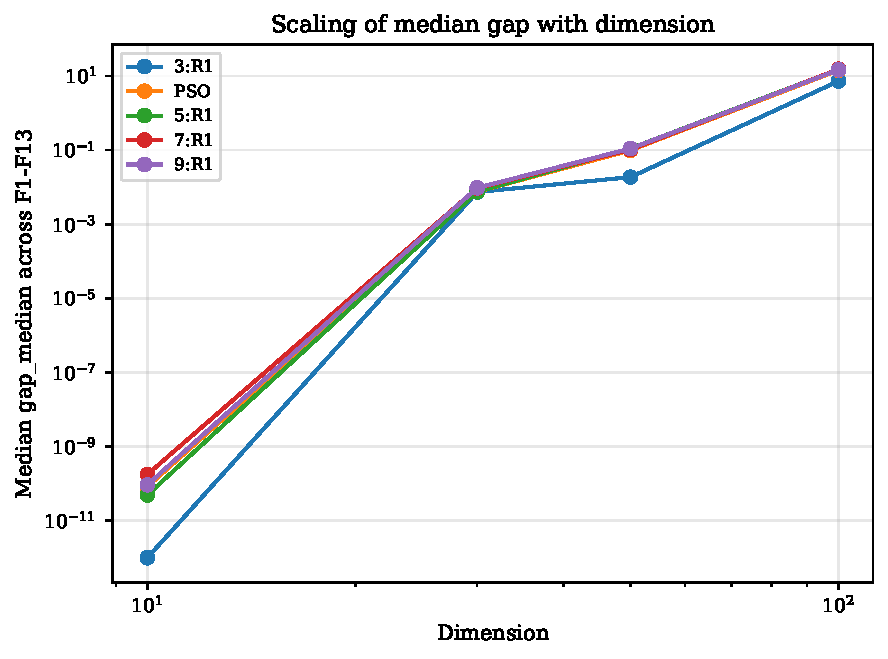
\includegraphics[width=0.85\linewidth]{figures/fig_scaling_curves.pdf}
  \caption{Median normalized gap versus dimension for the five highest mean-rank configurations on S1, including PSO. Both axes are logarithmic.}
  \label{fig:fig_scaling_curves}
\end{figure}

Runtime overhead is estimated as the ratio of independent sample medians for each configuration--instance group, without matching run identifiers. Across the 1,984 FCS--PSO group ratios, median overhead is 27.75\% (interquartile range: 19.81--50.94\%); the 32 configuration-level median ratios range from 25.79\% to 30.90\%. Function-level values in Table~\ref{tab:function_level} refer to the selected best-ranked FCS for that function; the large relative values on some inexpensive fixed-dimensional functions should not be interpreted as hardware-independent computational complexity. All execution times were measured in the same six-worker experiment environment.

\subsection{Dynamic behavior of the controller}
\label{subsec:results_dynamics}

The preceding subsections characterize what each configuration achieves; this one examines its behavior during optimization. Each run records the inertia weight and exploration percentage at every iteration. Exploration percentage (XPL) is defined as $100D_t/D_t^{\max}$, rounded to two decimal places, and corresponds to the normalized diversity ratio $d_t$ used as a controller input. XPL serves as an indicator of swarm dispersion rather than a direct measure of the relative contributions of exploration and exploitation to optimization performance. Figure~\ref{fig:fig_w_trajectories} presents the mean inertia weight and XPL across instances and runs, with XPL aligned to the pre-update swarm state used to compute each $w_t$.

The R1 mean trajectories decline over the run, but they are not the classical linear schedule. The baseline has mean inertia 0.500000 over iterations 0--1000; the existing run summaries give 0.499481, 0.499555, 0.499566, and 0.499835 for FCS-$n$-R1 at $n=3,5,7,9$, respectively. Despite these close overall means, the maximum absolute difference between each R1 mean trajectory and the observed PSO mean trajectory is 0.13480, 0.04194, 0.03315, and 0.02731, respectively. A direct 21-by-21 $(d,p)$ grid evaluation with the implemented controller ($n_{\mathrm{grid}}=501$) found maximum fixed-progress variation across diversity of 0.05325, 0.01160, 0.00973, and 0.00416 for those granularities. A convergence check on an 11-by-11 grid found that increasing the defuzzification grid from 501 to 1001 changed $w$ by less than $10^{-5}$; the observed diversity effects are therefore not numerical integration noise. R1 has diversity-invariant consequents but a weakly diversity-dependent, nonlinear effective schedule. Its leading rank does not establish a benefit of diversity feedback or equivalence to linear PSO. R2, its mirror, inverts the trajectory, while R5 and R6 produce other decreasing schedules and R7 and R8 increase inertia.

The aggregate profiles show a descriptive association between the early-to-late drop in $w$ and mean Friedman rank across the eight patterns (Spearman $\rho=-0.786$, $p=0.021$): patterns with larger declines tend to have better ranks. The end-of-run exploration percentage alone is not associated with rank ($\rho=0.21$, $p=0.61$). R4 and R8, the two patterns that retain the most exploration in the final hundred iterations (5.2\% and 3.6\%, respectively, versus roughly 0.6\% for R1, R3, R5, and R7), also do not converge. These summaries do not identify a causal mechanism; in particular, a nominally neutral consequent axis does not guarantee input independence under min--max inference.

Figure~\ref{fig:fig_convergence_representative} traces this into the convergence profile on four representative instances. On the unimodal F1 at $d=30$, \texttt{FCS-3-R1} remains below the baseline throughout and ends three orders of magnitude lower ($1.7 \times 10^{-9}$ against $7.7 \times 10^{-6}$), while \texttt{FCS-9-R2} stalls at $1.1 \times 10^{3}$ within the first two hundred iterations and never recovers: its weight is still rising when the budget ends. The same contrast appears on F14, where \texttt{FCS-3-R1} settles at a median of 1.99 against 3.97 for the baseline.

\startlandscape
\begin{figure}[H]
  \centering
  \includegraphics[width=\linewidth,height=0.82\textheight,keepaspectratio]{figures/fig_w_trajectories.pdf}
  \caption{Mean inertia weight $w_t$ (top) and normalized diversity XPL (bottom) by pattern and granularity, averaged over 62 instances and 31 runs. XPL is aligned to the pre-update state used for $w_t$. Colour and line style denote progress-consequent direction; PSO is shown as a linear-schedule reference.}
  \label{fig:fig_w_trajectories}
\end{figure}
\finishlandscape

\begin{figure}[!htbp]
  \centering
  \includegraphics[width=\textwidth]{figures/fig_convergence_representative.pdf}
  \caption{Median best fitness by iteration with interquartile bands over 31 runs for four representative instances. Panels compare PSO, \texttt{FCS-3-R1}, the function's best FCS when different, and \texttt{FCS-9-R2}; the vertical axis is symmetric-logarithmic.}
  \label{fig:fig_convergence_representative}
\end{figure}

These trajectories connect the leading ranks to the decreasing-progress consequent family, but do not show that R1 reproduces linear PSO or that its policy is driven solely by iteration progress. Its mean trajectory is nonlinear, and the effective R1 surface varies with diversity through the antecedent firing strengths. The results therefore concern the implemented Mamdani controllers, not an isolated comparison of time-only scheduling against diversity-state feedback.

The mechanism, however, does not imply universal dominance, for two reasons that the same figure makes explicit. On the scalable multimodal F9 at $d=30$, the configuration that wins most instances of that function, \texttt{FCS-5-R2}, descends faster than every alternative during the first two hundred iterations and reaches a median of 38.5, but it then stops improving entirely and finishes behind the baseline, which continues from 87.9 at iteration 200 down to 35.8. An aggressive early transition pays on functions where the budget is the binding constraint and costs on functions where it is not. On F23 the ordering reverses altogether: the baseline and \texttt{FCS-5-R6} both reach the optimum at $-10.54$, while \texttt{FCS-3-R1} stalls at $-3.84$, the same value as the last configuration of the study. A trajectory that is optimal on average is therefore not optimal everywhere, which is the dynamic counterpart of the per-instance heterogeneity of Section~\ref{subsec:results_function}: the 15 configurations that win at least one instance correspond to different ways of scheduling the transition, and none of them fits every landscape.

% Only four representative convergence cases are included in the article. Full trajectories
% remain in the iteration dataset; no separate Supplementary Information file is designated.
